%A Contratação Pública em Portugal pode ser classificada de duas formas: aberta e fechada. As regras presentes no Código dos Contratos Públicos (CCP) dizem respeito aos contratos públicos celebrados entre uma entidade adjudicante pública e uma entidade adjudicatária.

%sendo esta composta por atos e formalidades relativos à formação, conclusão e produção de uma plena eficácia jurídica de um contrato público. A eficácia jurídica - ao contrário da eficácia social - é um conceito teórico, segundo o qual uma norma definida de acordo com a lei se torna eficaz em termos jurídicos. \\

%O ato de adjudicar consiste em conferir o direito de algo a alguém, conceder algo ao maior licitante ou atribuir algo a alguém por concurso ou por ajuste. 
%Este é um termo essencial na área de contratação pública, sendo esta constituída pelas entidades adjudicantes e entidades adjudicatárias. 

%O CCP é aplicado a entidades adjudicantes públicas, tais como o Estado, Regiões Autónomas, Autarquias locais, Institutos públicos, Entidades Administrativas Independentes, Banco de Portugal, Fundações Públicas, Associações Públicas, Associações de que façam parte uma ou várias pessoas coletivas referidas anteriormente e que sejam maioritariamente financiadas por estas. Além destas, são consideradas entidades adjudicantes organismos de direito público, pessoas coletivas e associações \footnote{nos termos do artigo 2.º n.º 2, alíneas a), b) e d)}. São consideradas, também, entidades adjudicantes organismos com atuação nos setores especiais da água, energia, tranposrtes e serviços postais \footnote{artigo 7.º n.º 1.º}. Existe, também, a possibilidade de aplicar o CCP a entidades não adjudicantes que pretendem celebrar determinados contratos de empreitadas de obras públicas ou de serviços associados a obras \footnote{artigo 275.º}.


% Associações de que façam parte uma ou várias pessoas coletivas referidas anteriormente, desde que sejam maioritariamente financiadas por estas, estejam sujeitas ao seu controle de gestão ou tenham um órgão de administração, de direção ou de fiscalização cuja maioria dos titulares seja, direta ou indiretamente, designada pelas mesmas

% São ainda entidades adjudicantes organismos de direito público, pessoas coletivas e associações, independentemente da sua natureza pública ou privada, nos termos do artigo 2.º n.º 2, alíneas a), b) e d).

% Para além das entidades adjudicantes referidas no artigo 2º, são também entidades adjudicantes as referidas no artigo 7.º n.º 1.º, concretamente as pessoas coletivas que realizam atividades nos seguintes sectores especiais da água, energia, transportes e serviços postais.

% O CCP aplica-se ainda a entidades que não sendo adjudicantes, se encontrem nas situações previstas no artigo 275.º, ou seja, entidades que pretendam celebrar determinados contratos de empreitadas de obras públicas ou de serviços associados a obras, desde que estes contratos sejam subsidiados diretamente em mais de 50\% do respetivo preço contratual por entidades adjudicantes, sempre que o preço contratual for igual ou superior aos limiares comunitários.


%Existem duas fases principais no processo de contratação pública. 
%A primeira fase é a \textbf{fase preparatória} em que é feita a decisão de realizar um contrato e inclui uma fase preparatória do procedimento e uma fase instrutória que terminará no ato de ajudicação. A segunda fase é a \textbf{fase conclusiva} em que é concluído e celebrado o contrato. Existe também uma \textbf{fase complementar} que pode ser necessária na eventualidade do contrato público depender de atos posterioes à sua celebração tais como a aprovação, visto e publicidade. \\

\section{Código dos Contratos Públicos}

O Código dos Contratos Públicos (CCP) é o documento que estabelece um alinhamento com as diretivas comunitárias,  determinadas pelo Parlamento Europeu \cite{ue_dire}, definindo um conjunto homogéneo de normas relativas aos processos pré-contratuais e uma nova sistematização e uniformização de regimes substantivos dos contratos administrativos \cite{guia_poise}. Este documento encontra-se dividido em duas grandes categorias: \textbf{disciplina aplicável à contratação pública} e \textbf{regime substantivo dos contratos públicos}, correspondentes às Partes II e III do documento, respetivamente. O CCP pauta-se por um conjunto de objetivos gerais tal como ilustrado na Figura \ref{fig:ccpgoals}.

\begin{figure}[H]
	\centering
	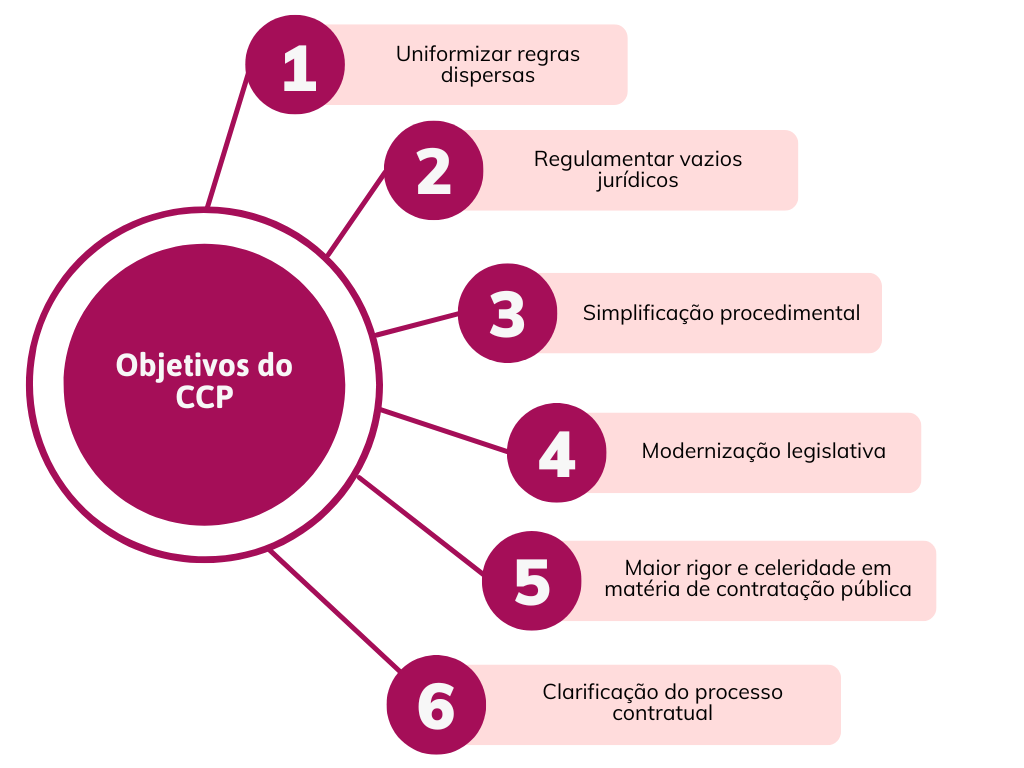
\includegraphics[width=0.5\textwidth]{imagens/ccp_objetivos.png}
	\caption{Objetivos gerais do Código dos Contratos Públicos.}
	\label{fig:ccpgoals}
\end{figure}


A simplificação da tramitação procedimental pré-contratual é feita através da implementação de novas tecnologias de informação/meios eletrónicos, incentivando a desburocratização, a desmaterialização, criando sistemas alternativos à utilização de papel e a simplificação da tramitação contratual.


Ao longo do processo contratual são definidos vários requisitos a cumprir:

\begin{my_enumerate}
	\item Qualificação dos candidatos;
	\item Métodos de avaliação;
	\item Valorização social e ambiental.
\end{my_enumerate}

Relativamente ao \textbf{nível de qualificação dos candidatos}, para determinadas tipologias de contrato, é exigido que os mesmos demonstrem possuir tanto capacidade técnica como financeira, a fim de completar o objeto contratual. 
É imperativo que os \textbf{métodos de avaliação de propostas}, componente crucial na formação e celebração de contratos públicos, sejam devidamente enunciados e publicitados, por forma a que as entidades concorrentes desenvolvam uma estratégia/proposta eficiente e a entidade adjudicante selecione, à luz desses mesmos critérios, a proposta mais vantajosa a nível económico, na ótica do interesse prosseguido. 
Além do mais, o CCP procura, de forma cabal, garantir que a enunciação e publicitação dos critérios de adjudicação e respetivos coeficientes de ponderação, se faça em conformidade com os princípos da igualdade, da concorrência, da imparcialidade, da proporcionalidade, da transparência, da publicidade e da boa fé.
É, também, necessário que o objeto do contrato a celebrar \textbf{reflita e valorize preocupações de cariz social e ambiental}\cite{ccp}\cite{guia_poise}. 

O incumprimento da legislação  que regula os procedimentos contratuais, pode implicar correções financeiras, cujas taxas são definidas em função da natureza e gravidade das irregularidades detetadas e, consequentemente, a uma perda de financiamento. As irregularidades que são detetadas com maior frequência encontram-se disponíveis para consulta na Tabela de Correções Financeiras COCOF \cite{corrections}\cite{cocoftab}.





\subsection{Entidades}

O artigo 2.º do CCP categoriza as entidades adjudicantes em dois organismos: organismos pertencentes ao setor público administrativo tradicional e organismos de direito público.


\begin{table}[h!]
	
	\centering
	\setlength{\tabcolsep}{15pt}
	\setlength\cellspacetoplimit{0.5cm} 
	\setlength\cellspacebottomlimit{0.5cm} 
	\renewcommand{\arraystretch}{1.5}

	\resizebox{\textwidth}{!}{
        \begin{tabular}{p{0.1\textwidth} p{0.1\textwidth} p{0.1\textwidth} p{0.25\textwidth} m{0.5\textwidth}} % Use p{} column type for vertical padding

			\hline
			\multicolumn{5}{Sc}{\textbf{Entidades Adjudicantes}} \\
			\hline
			\rowcolor[HTML]{EFEFEF} 
			\multicolumn{4}{Sc|}{\cellcolor[HTML]{EFEFEF}\textbf{Organismos pertencentes ao setor público administrativo tradicional}} & \textbf{Organismos de direito público} \\
			\hline
			Estado & Regiões Autónomas & Autarquias locais & Institutos públicos & \multirow{2}{=}{\centering Quaisquer pessoas coletivas que, independentemente da sua natureza pública ou privada, reúnam os requisitos presentes no n.º2 do artigo 2.º do CCP} \\ 
			Banco de Portugal & Fundações Públicas & Associações públicas & Entidades administrativas independentes & \\
			\hline
		\end{tabular}
	}
	
	\caption{Categorização das Entidades Adjudicantes.}
	\label{table:1}
\end{table}



Acresce às anteriormente menciondas outro tipo de entidades adjudicantes abrangidas pelo CCP pertencentes aos setores especiais da água, energia, transportes e serviços postais. 

A denominação  de \textit{entidade adjudicante} é válida, apenas, durante a fase pré-contratual. Após a celebração do contrato passa a denominar-se \textit{contraente público}. 



\subsection{Procedimentos para formação de contratos}
%\subsubsection{Equadramento Legal}

\subsubsection{Tipos de Procedimento e Contrato}
Os procedimentos pré-contratuais definidos no n.º1 do artigo 16.º do CCP, a serem adotados pelas entidades adjudicantes, encontram-se discriminados na Tabela \ref{table:2}.

\begin{table}[ht]
	\centering
	\renewcommand{\arraystretch}{1.15}
	\setlength{\tabcolsep}{15pt}
	%\resizebox{\textwidth}{!}{%
		\begin{tabular}{lc}
			\toprule
			\multicolumn{1}{c}{\textbf{Tipo de Procedimento}} & \textbf{Artigo do CCP} \\ 
			\midrule
			\rowcolor[HTML]{EFEFEF} 
			Ajuste Direto                                     & 112.º a 129.º          \\ 
			Consulta Prévia                                   & 112.º a 127.º          \\
			\rowcolor[HTML]{EFEFEF} 
			Concurso Público                                  & 130.º a 161.º          \\
			Concurso Limitado por Prévia Qualificação         & 162.º a 192.º          \\
			\rowcolor[HTML]{EFEFEF} 
			Diálogo Concorrencial                             & 204.º a 218.º          \\
			Procedimento de Negociação                        & 193.º a 203.º          \\
			\rowcolor[HTML]{EFEFEF} 
			Parceria para a Inovação                          & 218.º-A a 218.º-D      \\
			Acordos-quadro                                    & 251.º a 259.º          \\                             
			\bottomrule
		\end{tabular}
	%}
	\caption{Tipos de procedimento a adotar na fase pré-contratual.}
	\label{table:2}
\end{table}

Impõe-se, desde logo, uma descrição sumária de cada um dos procedimentos.

\begin{my_enumerate}
	
	%\item O \textbf{ajuste direto} consiste no convite direto, por parte da entidade adjudicante, a um operador económico à sua escolha, a fim de apresentar uma proposta para um determinado objeto contratual\cite{ajustedir}. Existem dois regimes para esta tipologia de procedimento: Ajuste Direto em Regime Geral e Ajuste Direto Simplificado. As diferenças entre estes dois regimes, que podem ser observadas na Tabela \ref{tab:4}, prendem-se com os valores contratuais máximos permitidos por lei.
	
	\item O \textbf{ajuste direto} corresponde ao procedimento de contratação pública em que a entidade adjudicante convida diretamente uma entidade à sua escolha para que esta apresente uma proposta\cite{ajustedir}. 
	
	Existem dois regimes para esta tipologia de procedimento: Ajuste Direto em Regime Geral e Ajuste Direto Simplificado. As diferenças entre estes dois regimes, consideradas na Tabela \ref{tab:4}, prendem-se com os valores contratuais máximos permitidos por lei.
	
	%\item Na \textbf{consulta prévia}, a entidade adjudicante convida diretamente, pelo menos, três operadores económicos à sua escolha a apresentar uma proposta. Os aspetos referentes ao contrato a celebrar podem ser negociados diretamente entre a entidade adjudicante e os operadores convidados \cite{consultaprev}. 
	
	\item A \textbf{consulta prévia} corresponde ao procedimento de contratação pública em que a entidade adjudicante convida diretamente, pelo menos, três entidades à sua escolha a apresentar proposta, podendo com elas negociar os aspetos da execução do contrato a celebrar\cite{consultaprev}. 
	
	
	%\item O \textbf{concurso público} pode ser adotado sempre que uma determinada entidade adjudicante o decidir. Não existe nenhuma fase prévia de qualificação dos concorrentes relativamente à capacidade técnico-financeira \cite{concursopub}. 
	
	\item O \textbf{concurso público} corresponde ao procedimento de contratação pública que é objeto de um anúncio num jornal oficial (Diário da República e/ou Jornal Oficial da União Europeia) no qual, qualquer entidade, que preencha os requisitos de participação, pode apresentar uma proposta\cite{concursopub}. 
	
	%\item O \textbf{concurso limitado por prévia qualificação} é adotado quando o valor do contrato a celebrar for superior aos limiares Europeus. Neste caso, o concurso é dado a conhecer, não só através do Diário da República, como nos itens anteriores, mas também no Jornal Oficial da União Europeia\cite{previaqual}. O \textbf{procedimento de negociação} partilha algumas características com este procedimento. 
	
	\item O \textbf{concurso limitado por prévia qualificação} corresponde ao procedimento de contratação pública que, sendo objeto de um anúncio num jornal oficial (Diário da República e/ou Jornal Oficial da União Europeia), se desdobra em 2 (duas) fases essenciais (qualificação e adjudicação), através das quais se constata se os candidatos preenchem os requisitos mínimos de capacidade definidos pela entidade adjudicante, sendo que os candidatos admitidos poderão, na segunda fase (adjudicação), apresentar uma proposta\cite{previaqual}.
	
	\item O \textbf{diálogo concorrencial} é utilizado nas situações em que a entidade adjudicante identifica uma necessidade e não sabe como satisfazer \cite{dialogoconc}. 
	
	\item A \textbf{parceria para a inovação} destina-se à realização de atividades de investigação e desenvolvimente de bens, serviços ou obras inovadoras. Tem como objetivo a aquisição destes bens desde que se cumpram os níveis de desempenho de preços máximos
	previamente combinados. Acontece quando um entidade adjudicante pretende adquirir um bem/serviço/obra
	pública com determinadas características que não se encontram no mercado. 
	
	%\item O \textbf{acordo quadro} é a celebração de um contrato entre uma ou várias entidades adjudicantes e uma ou mais entidades \cite{acordoquadro}. 
	
	\item O \textbf{acordo quadro} é a celebração de um contrato entre uma ou várias entidades adjudicantes e uma ou mais entidades \cite{acordoquadro}. 
	
	
\end{my_enumerate}

%Em ambos os casos existem limitações relativamente aos operadores económicos que podem ser convidados. (artigos 19.o, al. d), e 20.o, n.o 1, al. d), 19.o, al. c), e 20.o, n.o 1, al. c)). Não obstante, as limitações referidas não se aplicam em contratos ao abrigo de critérios materiais. 
%A celebração de consultas prévias e ajustes diretos deve ser publicitada no Portal dos Contratos Públicos pela entidade ajdudicante no prazo máximo de 20 dias a contar da data de celebração do contrato, a fim de comprovar a eficácia do respetivo contrato. 



%\textit{O CCP revê em alta ( o que é que isto significa? ) os limites relativos ao valor do contrato em função do procedimento pré-contratual adoptado. Para efeitos da determinação do valor do contrato, foi estabelecido que a escolha do procedimento condiciona o valor do contrato a celebrar. Por sua vez, o valor do contrato a celebrar pode ser entendido como o valor máximo do benefício económico obtido pelo adjudicatário com a execução de todas as prestações que constituem o objeto contratual.} \\



O n.º2 do artigo 16.º do CCP estabelece a tipologia do contrato a realizar, independentemente da sua natureza ou designação. As tipologias, \textit{empreitada de obras públicas} e \textit{concessão de obras públicas}\footnote{O n.º 2 do artigo 343.º do CCP define como obra pública qualquer trabalho de construção, reconstrução, ampliação, alteração ou adaptação, conservação, restauro, reparação, reabilitação, beneficiação e demolição de bens imóveis executados por conta de um contraente público.}, foram agregadas numa única categoria, doravante denominada \textit{Obras}\footnote{Ao longo deste texto irá ser utilizada tanto o termo Obras, como Empreitadas, para referir a presente tipologia de contrato.}. 
No que concerne às restantes tipologias, foram incluídas numa única categoria, doravante denominada \textit{Bens e Serviços}.

O artigo 135.º do supracitado código define o prazo mínimo, em dias, que as entidades concorrentes dispõem para apresentação de propostas relativas a cada umas das subcategorias de contratos. 

\begin{table}[h]
	\centering
	\resizebox{\textwidth}{!}{%
	\begin{tabular}{
			>{\columncolor[HTML]{FFFFFF}}l 
			>{\columncolor[HTML]{FFFFFF}}c 
			>{\columncolor[HTML]{FFFFFF}}c }
		\toprule
		\multicolumn{2}{c}{\cellcolor[HTML]{FFFFFF}\textbf{Tipo de Contrato}}                           & \textbf{\begin{tabular}[c]{@{}c@{}}Prazo mínimo para \\ apresentação de propostas\end{tabular}} \\ \midrule
		Empreitada de obras públicas        & \cellcolor[HTML]{FFFFFF}                                  & \cellcolor[HTML]{FFFFFF}                                                                 \\
		Concessão de obras públicas         & \multirow{-2}{*}{\cellcolor[HTML]{FFFFFF}Obras}           & \multirow{-2}{*}{\cellcolor[HTML]{FFFFFF}14 dias}                                        \\ \midrule
		Concessão de serviços públicos      & \cellcolor[HTML]{FFFFFF}                                  & \cellcolor[HTML]{FFFFFF}                                                                 \\
		Locação ou aquisição de bens móveis & \cellcolor[HTML]{FFFFFF}                                  & \cellcolor[HTML]{FFFFFF}                                                                 \\
		Aquisição de serviços               & \cellcolor[HTML]{FFFFFF}                                  & \cellcolor[HTML]{FFFFFF}                                                                 \\
		Sociedade                           & \multirow{-4}{*}{\cellcolor[HTML]{FFFFFF}Bens e Serviços} & \multirow{-4}{*}{\cellcolor[HTML]{FFFFFF}6 dias}                                         \\ 
		\bottomrule
	\end{tabular}%
	}
	\caption{Tipologia de contratos e respetivos prazos mínimos para apresentação de propostas por parte de entidades interessadas. }
	\label{table:3}
\end{table}

%Define-se, no  n.º 1 do artigo 343.º do CCP, \textbf{empreitada de obras públicas} como o contrato com objetivo de desenvolver e/ou executar uma obra pública inserida no regime de ingresso e permanência na actividade de construção. Por sua vez, no n.º 1 do artigo 407.º, é establecido que na \textbf{concessão de obras públicas} o co-contratante, obrigado, por lei, ao desenvolvimento e/ou execução do objeto contratual, tem direito a proceder, durante um determinado período de tempo, à exploração (da obra??) e, eventualmente, ao pagamento de um preço.
%Em suma, podem-se combinar os dois tipos de contratos anteriormente enunciados numa categoria definida como Obras. O n.º2 do artigo 343.º define como obra pública qualquer trabalho de construção, reconstrução, ampliação, alteração ou adaptação, conservação, restauro, reparação, reabilitação, beneficiação e demolição de bens imóveis executados por conta de um contraente público.

 




\subsubsection{Escolha do procedimento}

O artigo 36.º do CCP define que a escolha do tipo de procedimento, aquando da decisão de contratar, deve ser devidamente fundamentada. Antes da abertura de um procedimento de formação de contrato público, a entidade adjudicante pode efetuar consultas informais ao mercado a fim de poderem vir a ser utilizadas no planeamento da contratação. No caso dessa consulta ser efetuada a uma empresa que, posteriormente, se candidate ao concurso em questão, deve ser comunicada essa informação aos restantes concorrentes e incluí-la nas peças do procedimento\cite{guia_poise}.

Além disso, no momento da escolha do tipo de procedimento, devem ser considerados um de dois critérios: \textbf{critério do valor} e \textbf{critério material}. 
Ao optar pelo \textbf{critério do valor}, existem valores contratuais máximos consoante o tipo de procedimento, como se pode constatar na Tabela \ref{tab:4}. Define-se como valor do contrato, o valor máximo do benefício económico obtido pela entidade contratada após a completitude de todas as prestações que respeitam ao objeto contratual.

Se for elegido o \textbf{critério do valor}, nos termos do artigo 23.º do CCP, é permitida a celebração de contratos de qualquer valor. Para tal, é necessário que o órgão competente para a decisão de contratar, fundamente, de forma clara e objetiva, que os procedimentos adotados cumprem todos os requisitos previstos nos artigos 24.º a 30.º do CCP.




\subsubsection{Situações Excepcionais}


Aquando do desenvolvimento de contratos públicos existem algumas situações excepcionais, destacando-se a formação de \textbf{contratos mistos} e a \textbf{adjudicação por lotes}.
Os \textbf{contratos mistos} consistem num objeto contratual que contempla dois ou mais tipos de contrato diferentes\cite{mistos}, como por exemplo o \textit{fornecimento de bens móveis} e a \textit{prestação de serviços}.
A \textbf{adjudicação por lotes}, definida no artigo 46.º-A do CCP, consiste na divisão de um contrato financeiramente avultado, em vários contratos de valor inferior, sendo o número máximo de lotes estipulado pela entidade adjudicante. Desta forma, é permitida a participação de pequenas e médias empresas que não teriam capacidade organizacional e técnico-financeira adequada para a realização total do contrato. Na formação de contratos públicos de \textit{Bens e Serviços}, com um valor contratual superior a 135.000,00 €, a decisão de não contratação por lotes carece de obrigação de fundamentação, devendo respeitar os pontos inscritos no nr.º 2, do artigo 46.º-A, do CCP. Na formação de contratos públicos de \textit{Obras}, aplica-se o procedimento anteriormente mencionado nas situações em que o valor contratual é superior a 500.000,00 €. 


\begin{table}[h!]
	\renewcommand{\arraystretch}{1.6}
	\setlength{\tabcolsep}{15pt}
	\resizebox{\textwidth}{0.7\height}{%
	\begin{tabular}{ccccc}
		\hline
		\rowcolor[HTML]{C0C0C0} 
		\multicolumn{2}{c}{\cellcolor[HTML]{C0C0C0}\textbf{Tipo de Procedimento}}                                               & \textbf{Preço Base}                                                 & \textbf{Objeto} & \textbf{Base Legal (CCP)} \\ \hline
		\rowcolor[HTML]{FFFFFF} 
		\cellcolor[HTML]{FFFFFF}                                & \cellcolor[HTML]{FFFFFF}                                      & $\leq$ €10.000,00                                                   & Obras           & artigo 128.º, n.º1        \\
		\rowcolor[HTML]{FFFFFF} 
		\cellcolor[HTML]{FFFFFF}                                & \multirow{-2}{*}{\cellcolor[HTML]{FFFFFF}Regime Simplificado} & $\leq$ €5.000,00                                                    & Bens e Serviços & artigo 128.º, n.º1        \\ \cline{2-5} 
		\rowcolor[HTML]{FFFFFF} 
		\cellcolor[HTML]{FFFFFF}                                & \cellcolor[HTML]{FFFFFF}                                      & $\leq$ €30.000,00                                                   & Obras           & artigo 19.º, al d)        \\
		\rowcolor[HTML]{FFFFFF} 
		\cellcolor[HTML]{FFFFFF}                                & \cellcolor[HTML]{FFFFFF}                                      & $\leq$ €20.000,00                                                   & Bens e Serviços & artigo 20.º, n.º1, al c)  \\
		\rowcolor[HTML]{FFFFFF} 
		\multirow{-5}{*}{\cellcolor[HTML]{FFFFFF}Ajuste Direto} & \multirow{-3}{*}{\cellcolor[HTML]{FFFFFF}Regime Geral}        & $\leq$ €50.000                                                      & Outros          & artigo 21.º, n.º1, al c)  \\ \hline
		\rowcolor[HTML]{EFEFEF} 
		\multicolumn{2}{c}{\cellcolor[HTML]{EFEFEF}}                                                                            & $\leq$ €150.000,00                                                  & Obras           & artigo 19.º, al c)        \\
		\rowcolor[HTML]{EFEFEF} 
		\multicolumn{2}{c}{\cellcolor[HTML]{EFEFEF}}                                                                            & $\leq$  €75.000,00                                                  & Bens e Serviços & artigo 20.º, n.º1, al c)  \\
		\rowcolor[HTML]{EFEFEF} 
		\multicolumn{2}{c}{\multirow{-3}{*}{\cellcolor[HTML]{EFEFEF}Consulta Prévia}}                                           & $\leq$ €100.000                                                     & Outros          & artigo 21.º, n.º1, al c)  \\ \hline
		\rowcolor[HTML]{FFFFFF} 
		\multicolumn{2}{c}{\cellcolor[HTML]{FFFFFF}}                                                                            & \cellcolor[HTML]{FFFFFF}                                            & Obras           & artigo 19.º, al b)        \\
		\rowcolor[HTML]{FFFFFF} 
		\multicolumn{2}{c}{\cellcolor[HTML]{FFFFFF}}                                                                            & \multirow{-2}{*}{\cellcolor[HTML]{FFFFFF}Até aos Limiares Europeus*} & Bens e Serviços & artigo 20.º, n.º1, al b)  \\
		\rowcolor[HTML]{FFFFFF} 
		\multicolumn{2}{c}{\multirow{-3}{*}{\cellcolor[HTML]{FFFFFF}Concurso Público}}                                          & Qualquer valor                                                      & Outros          & artigo 21.º, n.º1, al a)  \\ \hline
	\end{tabular}%
	}
	\caption{Valores contratuais máximos permitidos por lei consoante a tipologia de procedimento e de contrato.}
	\label{tab:4}
\end{table}

Os Limiares Europeus são valores estabelecidos pela União Europeia que determinam a partir de que montante é obrigatório aplicar as normas europeias em matéria de contratação pública, variando consoante o tipo de contrato. Estes limiares são atualizados periodicamente e, para o ano de 2024, os valores a praticar são de $5.350.000,00$ € para \textit{Obras}. Para \textit{Bens e Serviços} este valor cai para os $140.000,00$ €, caso a entidade contratante seja uma autoridade governamental ou $431.000,00$ € caso a entidade contratante seja uma entidade do setor público.




\subsection{Tramitação Procedimental}

Na Figura \ref{fig:pecas} é possível visualizar, de uma forma simplista, as peças que são transversais a todos os tipos de procedimento contratual. 
São estas peças que definem as formalidades e requisitos que devem ser cumpridos na fase de elaboração e apresentação de propostas pelas entidades concorrentes. 
%\footnote{No caso do Ajuste Direto e Consulta Prévia não são tidas em conta as duas primeiras etapas. No Diálogo Concorrencial existem outras etapas intermédias.}
\begin{figure}[H]
	\centering
	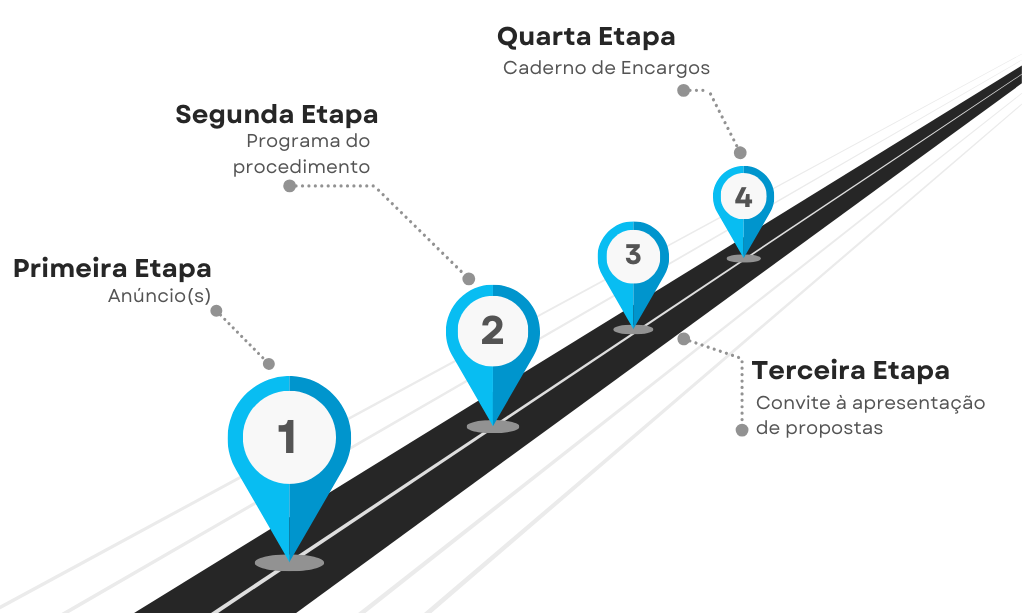
\includegraphics[width=0.55\textwidth]{imagens/pecasprocedimento.png}
	\caption{Ilustração das peças do procedimento de um concurso público.}
	\label{fig:pecas}
\end{figure}


O anúncio materializa-se em documento oficial, com base no qual a entidade adjudicante dá a conhecer ao mercado o início do procedimento de contratação pública. Este é obrigatoriamente publicado no Diário da República e, sob determinadas circunstâncias, no Jornal Oficial da União Europeia. \\
O programa do procedimento consiste no regulamento que define os termos que devem ser cumpridos desde a fase de formação do contrato até ao seu término\cite{programaproc}. \\
Por último, o caderno de encargos é a peça do procedimento onde estão definidas as cláusulas do contrato a celebrar \cite{caderno}. 
Na Figura \ref{fig:fasescp} é possível observar, com outro nível de detalhe, as fases constituintes da formação de um concurso público. 

\begin{figure}[H]
	\centering
	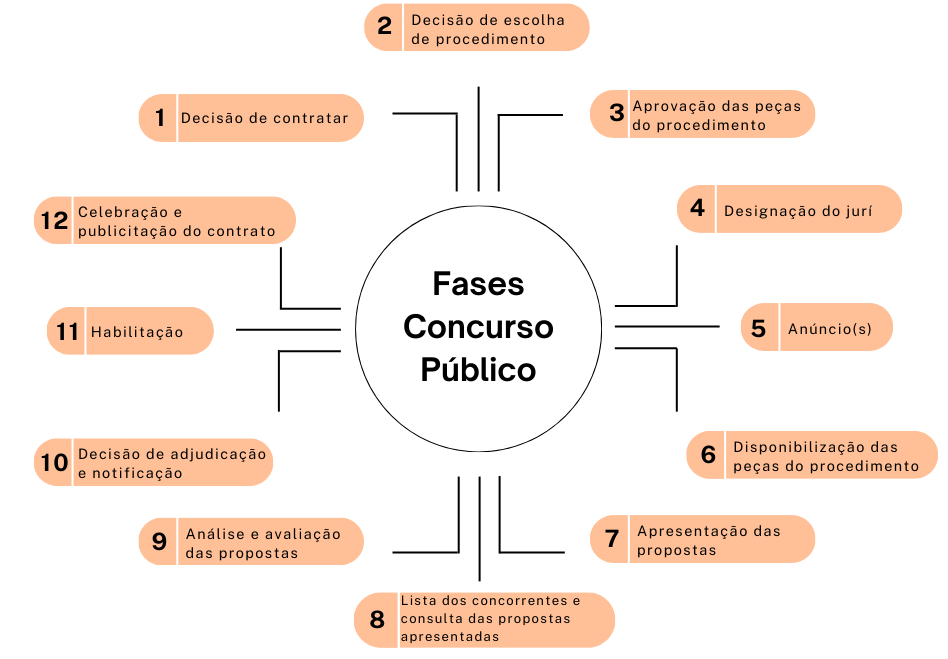
\includegraphics[width=.8\textwidth]{imagens/fasesconcpub.png}
	\caption{Fases do concurso público.}
	\label{fig:fasescp}
\end{figure}



